%
% Manchester Raspberry Jam Workshop Booklet
%
% This template is designed to try and aide consistency between each booklet.
% Insert files as instructed by comments, things like tables of contents are created by other linked files
%

% Is this document PRINT or WEB format?
% (you can use the toggle to cut content for paper, see etoolbox)
\newif\ifprint
\printfalse

% Page Formatting
\ifprint
	\documentclass[a4paper, twocolumn, twoside, 11pt]{article}
	\usepackage[margin=2cm]{geometry}
	\setlength{\columnsep}{1.25cm}
	\setlength{\parskip}{6pt}
\else
	\documentclass[a4paper, onecolumn, oneside, 11pt]{article}
	\usepackage[margin=3cm]{geometry}
	\setlength{\parskip}{9pt}
\fi



% FONT and text format
\usepackage[utf8x]{inputenc}	
\usepackage[UKenglish]{babel}
\ifprint
	\usepackage[usenames, dvipsnames]{color}				%Font Colour
	\usepackage[colorlinks=false]{hyperref}	%URLs
\else
	\usepackage[T1]{fontenc}
	\usepackage[sfdefault]{roboto}
	\usepackage[T1]{fontenc}
	\usepackage[usenames, dvipsnames]{color}				%Font Colour
	\usepackage[colorlinks=true,linkcolor=black,urlcolor=WildStrawberry]{hyperref}
\fi



% Table of Contents Format
\usepackage{tocloft}
\addtocontents{toc}{\cftpagenumbersoff{subsection}}
\setcounter{tocdepth}{2}
\setcounter{secnumdepth}{2}



% Section spacing
\ifprint
	\usepackage[compact]{titlesec}
\fi



% Listings and Asides
\usepackage{McrRaspJam/common/listings}
\usepackage{McrRaspJam/common/asides}



%Clear page for web version
\newcommand{\webclearpage}{
	\ifprint
	\else
		\clearpage
	\fi
}

% misc.
\usepackage{enumitem}									%List spacing changes
\usepackage[toc,page]{appendix}							%Appendix package
\usepackage{graphicx}									% TOC?
\usepackage{etoolbox}									%Boolean used for print/web switching
\usepackage{fancyvrb}									%Centered verbatim

% Enter the document title here
\newcommand{\workshopTitle}{Workshop 18: Games with Scratch}

% Enter the author of this workshop
\newcommand{\workshopAuthor}{Jack Kelly}


\begin{document}
	% Title Format
\ifprint
	\title{Manchester Raspberry Jam \\ \workshopTitle}
	\author{}
\else
	\title{
		\begin{center}
			
\includegraphics[width=30mm]{McrRaspJam/common/logo-512}
		\end{center}
		\vspace{12pt}
		\workshopTitle
	}
	\author{}
\fi

\date{\vspace{-32pt}}
\maketitle


% Online download location
\ifprint
	\begin{mdframed}[rightline=false, leftline=false]
		\scriptsize
		This booklet is available online at \mbox{\href{https://drive.google.com/open?id=0B_1SFjX_5JrmfnhpX0pPRXl6bmJNal8zdUxMeWZOdjJyZVdzU3V6UnBGdlVIMENtbFFkbVk}{bit.ly/McrRaspJam}}
		\normalsize
	\end{mdframed}
\fi
	
	%Place a SINGLE paragraph summary here
	In this workshop we'll recreate the classic arcade game \textit{Pong} in Scratch.
	
	%Difficulty
	\textit{Difficulty: Beginner workshop}

	\ifprint
		\renewcommand{\baselinestretch}{0.75}\normalsize
		\tableofcontents
		\renewcommand{\baselinestretch}{1.0}\normalsize
	\else
		\tableofcontents
	\fi
	
	%
	% Input the main CONTENT below, sans title page or contents.
	% Recommend inputting per section, and adding page breaks here.
	%
	% \webclearpage command is provided, will break page for web format only.
	%
	
	\setcounter{section}{-1}
\section{Introduction}
	
	%Difficulty
	%This is an introductory workshop.
		
	\subsection*{How to use these booklets}

	The aim of these booklets is to help you attempt these workshops at home, and to explain concepts in more detail than at the workshop. You don't need to follow these booklets during the workshop, but you can if you'd like 0to.
	
	%Code Listings
		The scratch code for this workshop will be shown in the booklet as images like the one shown in \autoref{fig:1followmouse1}.
	
	\begin{figure}[h]
		\centering
		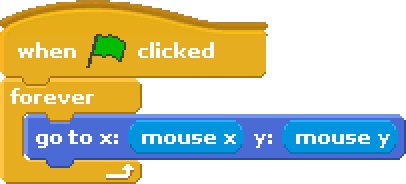
\includegraphics[height=69px]{McrRaspJam/018_ScratchGames/code/1_followmouse1}
		\caption{example code block}
		\label{fig:1followmouse1}
	\end{figure}
	%Occasionally, a concept will be explained in greater detail in \textit{asides}, like the one below. You can read these as you wish, but they're not required to complete the workshop.
	
\begin{aside}[API]
	We use an \textit{Application Programming interface} called `MCPI' to create Python programs for \textit{Minecraft: Pi Edition}.
	
	The API is a set of Python functions which allow us to communicate with the Minecraft game.
\end{aside}

	\subsection*{Everything else}
	
		\iffalse
	
		% Aknowledgements
		These booklets were created using \textrm{\LaTeX}, an advanced typesetting system used for several sorts of books, academic reports and letters.
			
		If you'd like to have a look at using LaTeX, We recommend looking at \TeX studio, which is available on most platforms, and also in the 	Raspbian repository.
		
		\fi
		
		% License spiel
		To allow modification and redistribution of these booklets, they are distributed under the \hbox{CC BY-SA 4.0} License.
		Latex source documents are available at \url{http://github.com/McrRaspJam/booklet-workshops}
		
		If you get stuck, find errors or have feedback about these booklets, please email me at:
		\href{mailto:jam@jackjkelly.com}{\texttt{jam@jackjkelly.com}}
		\pagebreak[3]
		
	%\section{Scratch}
	%\pagebreak[4]
		
	\section{Recreating Pong}

	\textit{Pong} was a very basic simulation of table tennis. Two players used \textbf{paddles} to bounce a \textbf{ball} back and forth across the screen. Points were scored when a player failed to hit an incoming ball with their paddle.
	
	Start by opening the template scratch file, which at the Jam will be found at \texttt{\textasciitilde{}/McrRaspJam/018\_ScratchGames/pong\_template.sb}. This template has the sprites for the two paddles and ball created for you.
	
	\begin{figure}[h]
		\centering
		
\includegraphics[width=0.4\linewidth]{McrRaspJam/018_ScratchGames/scrn/template}
		%\caption{The template file}
		\label{fig:template}
	\end{figure}


	\subsection{Player Paddle}
	
		In our version of Pong, you'll control the left paddle using the mouse, and the right paddle will be controlled by the computer.
		
		Each sprite in Scratch has its own code canvas, so \textbf{select} "Player" from the sprite list and then assemble the following code block.
		
		\begin{figure}[h!]
			\centering
			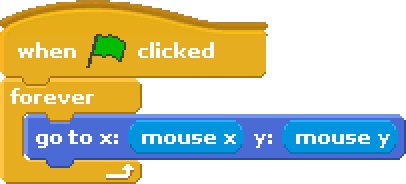
\includegraphics[height=69px]{McrRaspJam/018_ScratchGames/code/1_followmouse1}
			%\caption{Player paddle code}
			\label{fig:followmouse1}
		\end{figure}
		
		If you run your project, you will see that the paddle is now attached to the mouse cursor, but that's not quite what we want. In pong, the paddle follows the mouse up and down, but stays attached to the side of the screen.
		
		Choose one of the coordinates and remove the `mouse' block, and set it to a number instead. You should see the paddle now moves in one direction.
		
		To make the paddle move along the left side of the screen, the following code block is needed.
		
		\begin{figure}[h!]
			\centering
			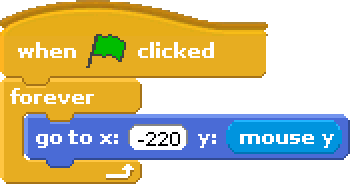
\includegraphics[height=69px]{McrRaspJam/018_ScratchGames/code/1_followmouse2}
			%\caption{Player paddle code}
			\label{fig:followmouse2}
		\end{figure}
		
	\subsection{Opponent Paddle}
	
		The right paddle will be controlled by the computer in this version of the game but don't worry, we don't need a complicated algorithm to play pong.
		
		\textbf{Select} the ``Opponent'' from the sprite list, and you should then see the blank code canvas for that sprite.
		
		Our computer paddle will have a very simple behaviour. It will simply look for the current position of the ball, then move towards it. We can get the position of the ball using the following code blocks.
		
		\begin{figure}[h!]
			\centering
			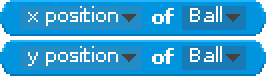
\includegraphics[height=38px]{McrRaspJam/018_ScratchGames/code/2_ballpos}
			%\caption{Code blocks for getting another sprite's position}
			\label{fig:ballpos}
		\end{figure}
	
		As with the player paddle, we're only going to change the y direction of the paddle. We'll start by creating a simple loop:
		
		\begin{figure}[h!]
			\centering
			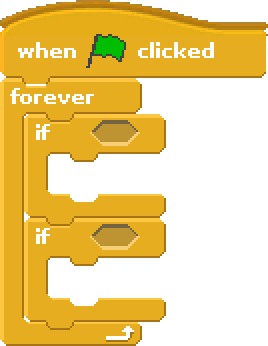
\includegraphics[height=130px]{McrRaspJam/018_ScratchGames/code/2_loop}
			\label{fig:opponentloop}
		\end{figure}
	
		Each time the loop runs, we'll check if the ball is higher than the paddle, and move the paddle up if that is true.
		
		\begin{figure}[h!]
			\centering
			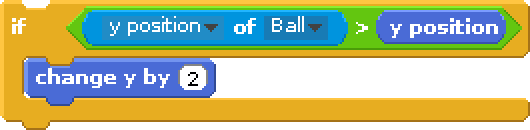
\includegraphics[height=49px]{McrRaspJam/018_ScratchGames/code/2_if1}
			\label{fig:opponentif1}
		\end{figure}
		
		Then we'll check if the ball is lower than the paddle, and move the paddle down if that is true.
		
		\begin{figure}[h!]
			\centering
			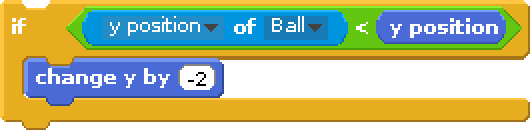
\includegraphics[height=49px]{McrRaspJam/018_ScratchGames/code/2_if2}
			\label{fig:opponentif2}
		\end{figure}
	
		You should also set the initial position of the paddle to \texttt{x = 220} before the \texttt{forever} loop so the paddle is placed on the right side of the screen.
		
		Run your game, and move the ball around by clicking and dragging to test whether the paddle is working.
		
	\subsection{The Ball}
	
		\textbf{Select} the Ball from the sprite list, you should once again see a blank code canvas.
		
		\subsubsection{Moving the Ball}
		
			We're going to control the ball by storing the \texttt{x} and \texttt{y} speeds of the ball. Create two sprite variables, which I have called \texttt{BallSpeedX} and \texttt{BallSpeedY}.
			
			Create a new code block, and set the speeds of the ball to some number.
			
			\begin{figure}[h!]
				\centering
				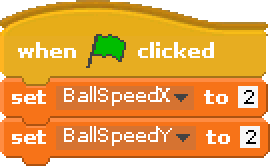
\includegraphics[width=101px]{McrRaspJam/018_ScratchGames/code/3_ballmove1}
				\label{fig:ballmove1}
			\end{figure}
		
			Then add a simple loop and move the ball using the variable values.
			
			\begin{figure}[h!]
				\centering
				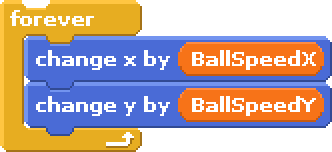
\includegraphics[width=125px]{McrRaspJam/018_ScratchGames/code/3_ballmove2}
				\label{fig:ballmove2}
			\end{figure}
		
			If you run your program now, depending on the numbers you used, the ball will probably move into one of the corners and get stuck. Next, we need to make the ball bounce.
			
			\iffalse
				\begin{figure}[h]
					\centering
					
\includegraphics[width=0.4\linewidth]{McrRaspJam/018_ScratchGames/scrn/ballmove1}
					\caption{The Ball getting stuck on an edge}
					\label{fig:ballmovescreen}
				\end{figure}
			\fi
		
		\subsubsection{Bouncing (top/bottom)}
		
			if the ball hits the top or bottom edge of the screen, we want it to `reflect' in the other direction. Because our ball movement uses x and y speeds, we can just inverse one of these values to make the ball bounce.
			
			By moving your mouse around the game screen and reading the coordinate output on the screen you should be able to see that the screen goes from -240 to 240 on the x axis and -180 to 180 on the Y axis.
			
		    We'll change the direction of the ball whenever it's near the edge of the screen. To do this create another loop with if statements.
			
			\begin{figure}[h!]
				\centering
				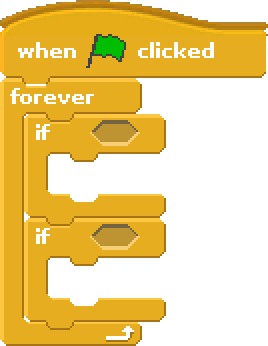
\includegraphics[width=101px]{McrRaspJam/018_ScratchGames/code/2_loop}
				\label{fig:ballloop}
			\end{figure}
			
			If the ball reaches the top ten pixels of the screen, we'll make it point downwards. We'll do the opposite if the ball reaches the bottom of the screen.
			
			\begin{figure}[h!]
				\centering
				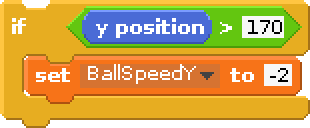
\includegraphics[width=116px]{McrRaspJam/018_ScratchGames/code/3_ballbounce1}
				\label{fig:ballbounce1}
			\end{figure}
		
			\begin{figure}[h!]
				\centering
				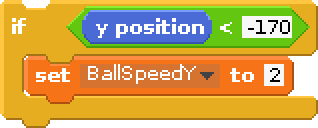
\includegraphics[width=116px]{McrRaspJam/018_ScratchGames/code/3_ballbounce2}
				\label{fig:ballbounce2}
			\end{figure}
		
		\subsubsection{Bouncing off paddles (left/right)}
		
			We can start off the horizontal bounces in a similar way. If we wanted the ball to bounce off the right side of the screen, we could use the following if statement.
		
			\begin{figure}[h!]
				\centering
				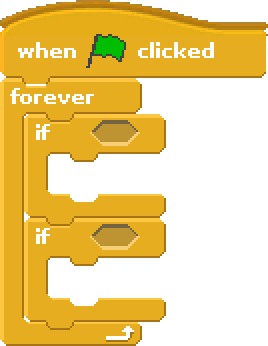
\includegraphics[width=101px]{McrRaspJam/018_ScratchGames/code/2_loop}
				\label{fig:ballloop2}
			\end{figure}
		
			\begin{figure}[h!]
				\centering
				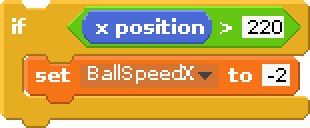
\includegraphics[width=116px]{McrRaspJam/018_ScratchGames/code/4_paddle1}
				\label{fig:paddle1}
			\end{figure}
		
			\pagebreak[4]
			However, we only want the ball to bounce if it's touching the opponents paddle. We'll do this by placing an if/else block inside the if block.
			
			\begin{figure}[h!]
				\centering
				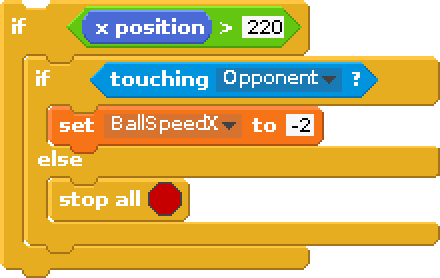
\includegraphics[width=165px]{McrRaspJam/018_ScratchGames/code/4_paddle2}
				\label{fig:paddle2}
			\end{figure}
			
			Now, the ball only bounces if it's touching the paddle. If it isn't, the opponent has lost, and for now we'll stop the game using a stop all command.
			
			Create the matching block for the left-hand side of the screen. You should then be able to play a single round of the game.
			
	\subsection{Resetting and Scoring}
	
		\textit{This section will be added after the Jam}
	
\end{document}